\documentclass{article}
\usepackage{tikz}
\usetikzlibrary{arrows.meta,positioning,calc,shapes.geometric}
\pagestyle{empty}
\begin{document}
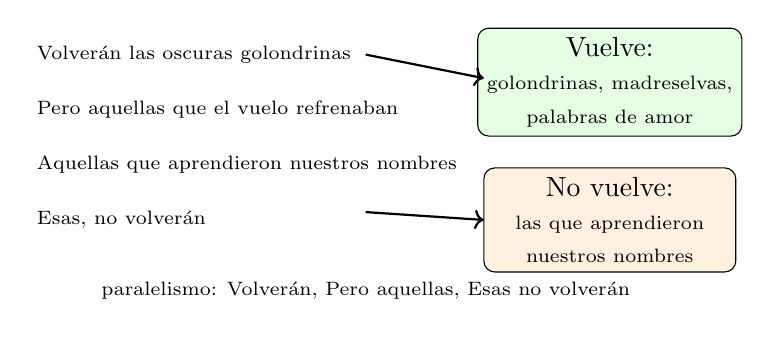
\begin{tikzpicture}
\tikzset{every node/.append style={align=center}}

\node[font=\scriptsize, anchor=west] at (0.2,3.2) {Volverán las oscuras golondrinas};
\node[font=\scriptsize, anchor=west] at (0.2,2.5) {Pero aquellas que el vuelo refrenaban};
\node[font=\scriptsize, anchor=west] at (0.2,1.8) {Aquellas que aprendieron nuestros nombres};
\node[font=\scriptsize, anchor=west] at (0.2,1.1) {Esas, no volverán};
\node[draw, rounded corners, fill=green!10, minimum width=3.2cm, align=center] at (7.6,2.85) {Vuelve:\\ \scriptsize golondrinas, madreselvas,\\ \scriptsize palabras de amor};
\node[draw, rounded corners, fill=orange!12, minimum width=3.2cm, align=center] at (7.6,1.1) {No vuelve:\\ \scriptsize las que aprendieron\\ \scriptsize nuestros nombres};
\draw[->, thick] (4.5,3.2) -- (6.0,2.9); \draw[->, thick] (4.5,1.2) -- (6.0,1.1);
\node[font=\scriptsize] at (4.5,0.2) {paralelismo: Volverán, Pero aquellas, Esas no volverán};

\end{tikzpicture}
\end{document}
